\documentclass[12pt,twoside, letter]{exam}
\usepackage{enumitem, kantlipsum}
\usepackage[margin=1in,left=1in,right=1in,top=1in,bottom=1in]{geometry}
\usepackage{graphicx,epstopdf}
\usepackage{amssymb,amsmath,amsfonts, amsthm}
\usepackage{wasysym}
\newtheorem{theorem}{Theorem}
\newtheorem{corollary}{Corollary}[theorem]
\newtheorem{lemma}[theorem]{Lemma}
\usepackage{hyperref}
\usepackage{tikz}
\usepackage{xstring}
\usetikzlibrary{calc}
\usepackage{ducksay}
\newtheorem{prop}{Proposition}

\theoremstyle{definition}
\newtheorem{definition}{Definition}

\usepackage{bbm}
\usepackage{verbatim}
\usepackage{bbold}
\usepackage{phfparen}
\usepackage{sets}
\newcommand{\nn}{\mathbb{N}}
\newcommand{\rr}{\mathbb{R}}
\newcommand{\cc}{\mathbb{C}}
\newcommand{\cb}{\mathcal{B}}
\newcommand{\ctau}{\mathcal{T}}
\newcommand{\co}{\mathcal{O}}
\newcommand{\zz}{\mathbb{Z}}
\newcommand{\ee}{\mathbb{E}}
\newcommand{\qq}{\mathbb{Q}}
\newcommand{\interior}{\text{Int}}
\newcommand{\pp}{\mathbb{P}}
\newcommand{\id}{\mathbbm{1}}
\newcommand{\Co}{\text{Co}}
\newcommand{\Cl}{\text{Cl}}
\usepackage{mathtools}
\DeclarePairedDelimiter\ceil{\lceil}{\rceil}
\DeclarePairedDelimiter\floor{\lfloor}{\rfloor}


\usepackage{indentfirst}
\setlist{
    listparindent = \parindent,
    parsep = 6pt,
}

\makeatletter
\newsavebox\myboxA
\newsavebox\myboxB
\newlength\mylenA

\newcommand*\xoverline[2][0.9]{%
    \sbox{\myboxA}{$\m@th#2$}%
    \setbox\myboxB\null% Phantom box
    \ht\myboxB=\ht\myboxA%
    \dp\myboxB=\dp\myboxA%
    \wd\myboxB=#1\wd\myboxA% Scale phantom
    \sbox\myboxB{$\m@th\overline{\copy\myboxB}$}%  Overlined phantom
    \setlength\mylenA{\the\wd\myboxA}%   calc width diff
    \addtolength\mylenA{-\the\wd\myboxB}%
    \ifdim\wd\myboxB<\wd\myboxA%
       \rlap{\hskip 0.5\mylenA\usebox\myboxB}{\usebox\myboxA}%
    \else
        \hskip -0.5\mylenA\rlap{\usebox\myboxA}{\hskip 0.5\mylenA\usebox\myboxB}%
    \fi}
\makeatother

\usepackage{float}
\floatstyle{boxed}
\restylefloat{figure}

\printanswers

\begin{document}


\abovedisplayskip=12pt
\belowdisplayskip=12pt
\abovedisplayshortskip=7pt
\belowdisplayshortskip=10pt
\allowdisplaybreaks

\setlength{\parindent}{18pt}

\title{Quantitative Methods: Assignment 3}
\author{Raymond Luo}
\date{\today}
\maketitle

\noindent {\bf Problem 1 (25 points):}
\par{Implement a program in Matlab to compute numerically the steady state of the airline problem seen in class. Provide a printout of your code and
a summary of your results}
\begin{solution}
  \begin{figure}[H]
    \centering
      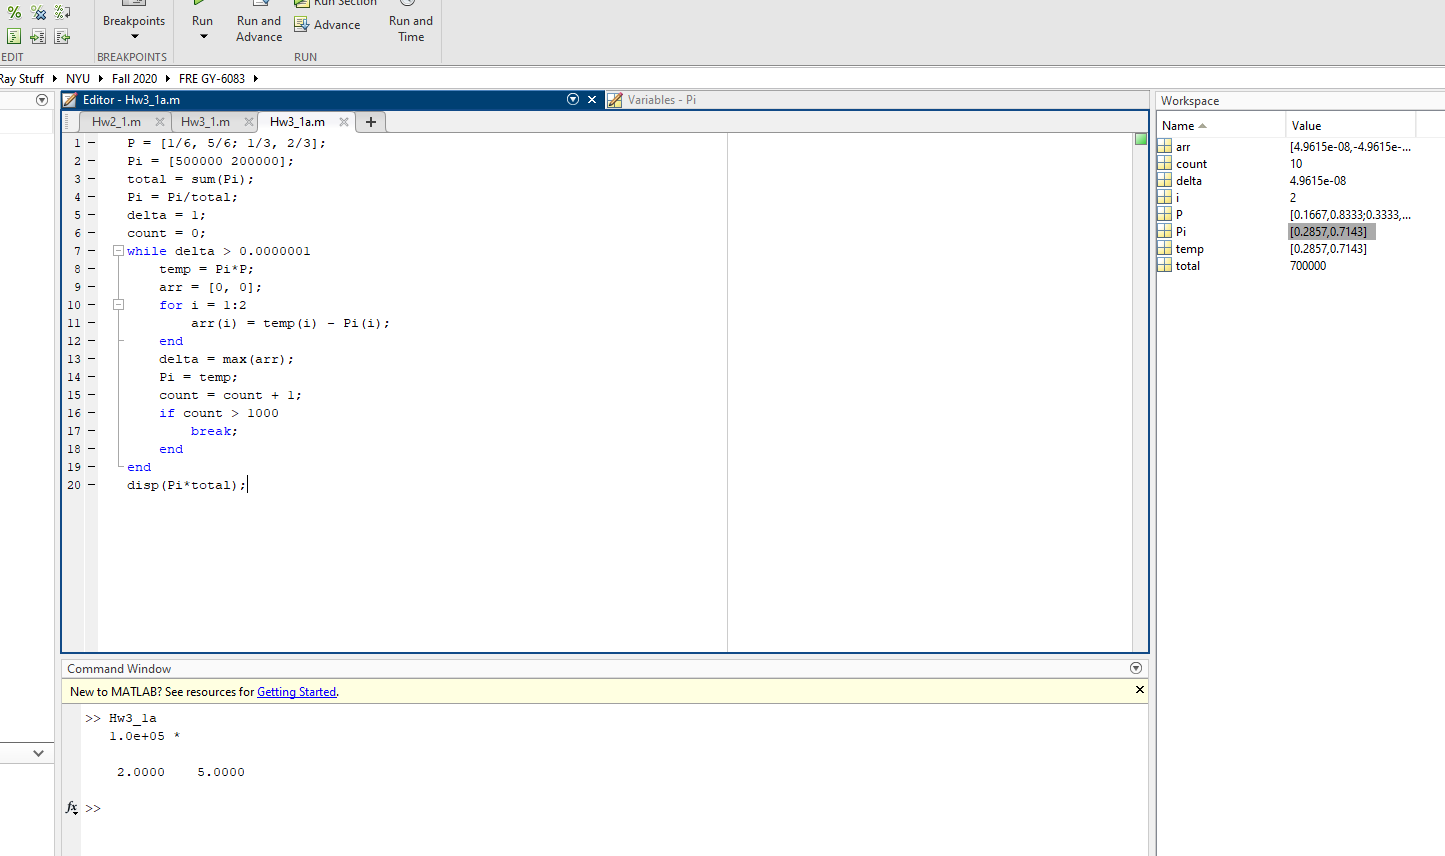
\includegraphics[width=5in]{Hw3_1a}
  \end{figure}
\end{solution}


\noindent {\bf Problem 2 (20 points):}
\par{Consider a Markov chain $X_{n}$ with state space $\{0,1,2 \}$ and one-step transition probability matrix }

\begin{align*}
  \centering
  P =
    \begin{bmatrix}
      1/2 & 1/4 & 1/4 \\
      \alpha & 0 & 1 - \alpha \\
      \beta & 0 & 1- \beta
    \end{bmatrix}
\end{align*}
  \begin{enumerate}
    \item For what values of $\alpha$ and $\beta$ is the Markov chain irreducible?

      \begin{solution}
        We note that as state 0 has a nonzero probability of transitioning to states 1 and 2. It is sufficient for states 1 and 2 to have a nonzero probability of transitioning to
        state 0 to be irreducible. As state 2 transitions to state 0 if and only if $\beta \neq 0$ and state 1 transitions to either state 0 or 2 for all values of $\alpha$, we have an
        irreducible Markov chain if $\alpha \in [0,1], \beta \in (0,1]$
      \end{solution}

    \item Suppose that $\alpha = 1/2$, $\beta = 1/4$. Solve the following question experimentally, using Matlab: Do the limiting probability
      $\pi_{j}$ exist for $j = 0,1,2$? \\
      Solution:
        \begin{figure}[H]
          \centering
            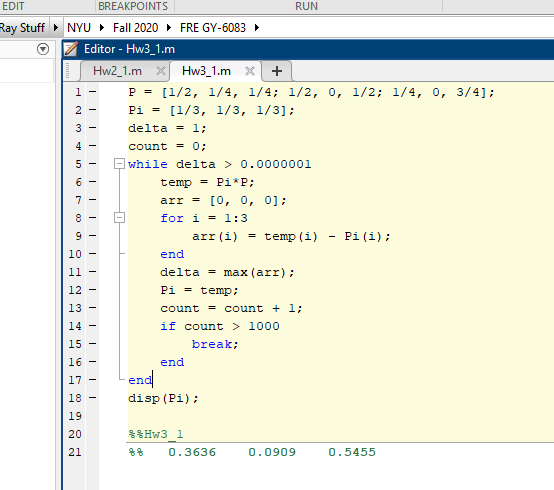
\includegraphics[width=2in]{Hw3_1b}
        \end{figure}

    \item Solve the system of linear equations
      \begin{equation*}
        \pi = \pi P
      \end{equation*}
      Compare the solutions with the limit you found in the previous question.
      \begin{solution}
        Suppose $\pi = (x_1 \quad x_2 \quad x_3)$ so that \\
        $\pi P = (1/2x_1 + \alpha x_2 + \beta x_3 \qquad 1/4x_1 \qquad 1/4x_1 + (1-\alpha)x_2 + (1-\beta)x_3)$ \\
        As $\alpha = 1/2, \beta = 1/4$, we have system of equations:
          \begin{align*}
            &x_1 = 1/2x_1 + 1/2 x_2 + 1/4 x_3 \\
            &x_2 = 1/4x_1 \\
            &x_3 = 1/4x_1 + 1/2 x_2 + 3/4x_3 \\
            &x_1 + x_2 + x_3 = 1 \text{ condition that $\pi \cdot \id = 1$}
          \end{align*}
        So we get $\pi = (4/11 \quad 1/11 \quad 6/11)$ \\
The answers are approximately the same as the ones we found through matlab simulation. Truncation error can be controlled through the conditions of our for loop.s
      \end{solution}
  \end{enumerate}

\noindent {\bf Problem 3 (10 points)}
\par{The one-step transition probability matrix $P$ of a Markov chain with state space $\{0,1\}$ is given by}
\begin{align*}
  \centering
  P =
    \begin{bmatrix}
      1/4 & 3/4 \\
      1/2 & 1/2 \\
    \end{bmatrix}
\end{align*}
Assume that $\pp[X_0 = 0] = 1/3$. Calculate $\ee[X_2]$

\begin{solution}
  We have that $\pp[X_0 = 0] = 1/3, \pp[X_0 = 1] = 1-\pp[X_0 = 0] = 2/3$. We denote this by $\pi = (1/3 \quad 1/2)$.
  We then note that $\ee[X_2] = \pi \cdot P^{2}$. \\

  \begin{align*}
    \centering
    P^2 =
      \begin{bmatrix}
        (1/4)^2+3/4\cdot 1/2 & 1/4 \cdot 3/4 + 3/4 \cdot 1/2 \\
        1/4 \cdot 1/2 + (1/2)^2 & 1/2 \cdot 3/4 + (1/2)^2 \\
      \end{bmatrix}
      =
      \begin{bmatrix}
        7/16 & 9/16 \\
        6/16 & 10/16 \\
      \end{bmatrix}
  \end{align*}
  So we have that $\pi \cdot P^2 = (19/48 \quad 29/48)$
\end{solution}


\noindent{\bf Problem 4 (15 points)}
\par{Consider the gambler's ruin problem with $k=5$ and the initial capital $i=2$}

\begin{enumerate}
  \item Suppose that, on any given round of the game, the gambler has a probability of 1/2 of winning one dollar, a probability of
    1/4 of losing one dollar, and a probability of 1/4 of neither winning nor losing. Give the state space and the transition probability matrix $P$ of the
    Markov chain representing the gambler's total wealth.
    \begin{solution}
      The state space $S = \{0, 1, 2, 3, 4, 5\}$ represents the wealth we can have at a time $n$. \\
      Our transition probability matrix is:
      \begin{align*}
        \centering
        P =
          \begin{bmatrix}
            1 & 0 & 0 & 0 & 0 & 0 \\
            1/4 & 1/4 & 1/2 & 0 & 0 & 0 \\
            0 & 1/4 & 1/4 & 1/2 & 0 & 0\\
            0 & 0 & 1/4 & 1/4 & 1/2 & 0 \\
            0 & 0 & 0 & 1/4 & 1/4 & 1/2 \\
            0 & 0 & 0 & 0 & 0 & 1
          \end{bmatrix}
      \end{align*}
      We have initial wealth represented by matrix $\pi = (0 \quad 0 \quad 1 \quad 0 \quad 0  \quad 0)$
    \end{solution}
  \item Can you characterize the probability of ruin? Can you compute it? Hint: to some extent, you many follow the approach seen in class. However, your calculations do not need to be
    as general as in the lecture notes since both the initial and target capital are set to specific values in this exercise. Of course, you also need to be aware that, unlike
    in the lecture notes, there is a positive probability of neither winning nor losing.
      \begin{solution}
        We note that the probability of ruin at any given time $t$ is given by $\big[ \pi\cdot P^{t} \big]_{(0)}$ and that $\pp[\text{Ruin}] = \lim_{n \rightarrow \infty} \big[\pi P^{n}\big]_{(0)}$.\\
        We proceed by the following construction: For $n \in [1,k]$, $P_{n} = \pp[\text{ Ruin } \mid X_{0} = i]$ where $X_{t}$ denotes the amount of money we have at time $t$. \\
        Note that $P_{n} = \pp[\text{ Ruin } \mid X_{0} = i] \\
        = \pp[\text{ Ruin } \cap \text{"First bet is a win"} \mid X_{0} = i] + \pp[\text{ Ruin } \cap \text{"First bet has no change"} \mid X_{0} = i]
        + \pp[\text{ Ruin } \cap \text{"First bet is a loss"} \mid X_{0} = i] \\
        = \pp[\text{Win}]\pp[\text{ Ruin } \mid X_{1} = i+1] + \pp[\text{Tie}]\pp[\text{ Ruin } \mid X_{1} = i]
        + \pp[\text{Loss}]\pp[\text{ Ruin } \mid X_{1} = i-1] \\
        = \pp[\text{Win}]\pp[\text{ Ruin } \mid X_{0} = i+1] + \pp[\text{Tie}]\pp[\text{ Ruin } \mid X_{0} = i]
        + \pp[\text{Loss}]\pp[\text{ Ruin } \mid X_{0} = i-1] \\
        = \frac{1}{2} P_{n+2} + \frac{1}{4} P_{n+1} + \frac{1}{4} P_{n}$ \\
        We then have a recurrence relation $P_{n+1} = \frac{1}{2} P_{n+2} + \frac{1}{4} P_{n+1} + \frac{1}{4} P_{n} \Rightarrow 3P_{n+1} = P_{n+2} + 2P_{n}$ with $P_{0} = 1, P_{k} = 0$.
        We solve the recurrence relation by using the characteristics equation $2r^2 -3r+1=(2r-1)(r-1)=0$:
        \begin{align*}
          \text{We then know that our above relation has closed form:} \\
          P_{n} &= A\cdot (\frac{1}{2})^n + B \cdot (1)^n. \\
          P_{0} &= A + B = 1 \\
          P_{5} &= A\cdot \frac{1}{32} + B = 0 \\
          \Rightarrow A &= \frac{32}{31}, B = \frac{-1}{31} \\
          P_{n} &= \frac{32\cdot \frac{1}{2^n}-1}{31} \\
          \Rightarrow \text{$\pp[\text{Ruin} \mid i = 2]$} = P_{2} = \frac{7}{31}
        \end{align*}
      \end{solution}
\end{enumerate}

\noindent{\bf Problem 5 (30 points)}
\par{Consider the Markov chain with state space $\{0,1,2\}$ and transition probability matrix}

\begin{align*}
  \centering
  P =
    \begin{bmatrix}
      0 & 1/2 & 1/2 \\
      1/3 & 0 & 2/3 \\
      1/2 & 1/2 & 0
    \end{bmatrix}
\end{align*}

\begin{enumerate}
  \item Show that this chain is irreducible
    \begin{solution}
      We note that from state 0, we have nonzero probability of transitioning to state 1 and 2. We note that from state 1, we have nonzero probability of transitioning to state 2 and 3.
      We note that from state 2, we have nonzero probability of transitioning to state 0 and 1. It is immediate that this chain is irreducible.
    \end{solution}
  \item Compute $P^2$ and $P^3$
    \begin{solution}
      \begin{align*}
        \centering
        P^2 =
          \begin{bmatrix}
            1/2\cdot 1/3 + 1/2 \cdot 1/2 & 1/2 \cdot 1/2 & 1/2 \cdot 2/3 \\
            1/2 \cdot 2/3 & 1/2 \cdot 1/3 + 1/2 \cdot 2/3 & 1/3 \cdot 1/2 \\
            1/3 \cdot 1/2 & 1/2 \cdot 1/2& 1/2 \cdot 1/2 + 1/2 \cdot 2/3
          \end{bmatrix}
            =
            \begin{bmatrix}
              5/12 & 1/4 & 1/3 \\
              1/3 & 1/2 & 1/6 \\
              1/6 & 1/4 & 7/12
            \end{bmatrix}
      \end{align*}
      \begin{align*}
        \centering
        P^3 =
            \begin{bmatrix}
              1/4 & 3/8 & 3/8 \\
              1/4 & 1/4 & 1/2 \\
              3/8 & 3/8 & 1/4
            \end{bmatrix}
      \end{align*}
    \end{solution}
  \item Deduce that the chain is aperiodic
    \begin{solution}
      It suffices to show that $\forall i \in \{0,1,2\}, \forall n \geq N$ for some $N < \infty$, that $(P^{n})_{i,i} > 0$.
      We note that for $N = 2$, $(P^{N})_{i,i} > 0$ for all $i \in \{0,1,2\}$. We proceed by strong induction.
    \end{solution}
  \item Is the chain ergodic? Justify your answer
    \begin{solution}
      Ergodicity follows from the fact that the chain is both aperiodic and irreducible.
    \end{solution}
  \item Determine the ergodic limit $\pi$.
    \begin{solution}
      We first note that ergodicity ensures the existence of limit $\pi$. Thus, we assume that $\pi = (x_1, x_2, x_3)$ such that
      $\pi = \pi \cdot P$. We then have the following system of equations:
        \begin{equation}
          x_1 = \frac{1}{3} x_2 + \frac{1}{2} x_3
        \end{equation}
        \begin{equation}
          x_2 = \frac{1}{2} x_1 + \frac{1}{2} x_{3}
        \end{equation}
          (2) substituted into $3*$(1) gives us:
        \begin{equation}
          3x_1 = \frac{1}{2}x_1 + \frac{1}{2}x_3 + \frac{3}{2}x_3 \Rightarrow x_1 = \frac{4}{5}x_3
        \end{equation}
      As we know that $x_1 + x_2 + x_3 = 1$, (2) substituted into this equation with (3) gives us:
        \begin{equation}
          1-x_1 - x_3 = \frac{1}{2}x_1 + \frac{1}{2}x_{3} \Rightarrow x_3 = \frac{10}{27}, x_{1} = \frac{8}{27}
        \end{equation}
      We then have that $\pi = (\frac{8}{27} \quad \frac{1}{3} \quad \frac{10}{27})$
    \end{solution}
\end{enumerate}


\end{document}
